\section{实验一:运算器组成实验}
    \subsection{实验目的及任务}
        \begin{itemize}
            \item 实验目的:
            \begin{enumerate}
                \item 熟悉 \textit{TEC-}8 模型计算机的节拍脉冲 \textit{T}1、\textit{T}2、\textit{T}3
                \item 熟悉双端口通用寄存器组的读写操作
                \item 熟悉运算器的数据传送通路
                \item 熟悉 \textit{ALU} (74\textit{LS}181) 的加减与或功能 
            \end{enumerate}
            \item 实验任务:
            \begin{enumerate}
                \item 熟悉手工连线方式:完成控制信号模拟开关与运算模块的外部连线
                \item 熟悉利用数据开关向通用寄存器 \textit{R}3-\textit{R}0 中置入数据
                \item 验证 \textit{ALU} 的算术运算和逻辑运算功能
            \end{enumerate}
        \end{itemize}

    \subsection{实验电路分析}
        \begin{figure}[htbp]
            \centering
            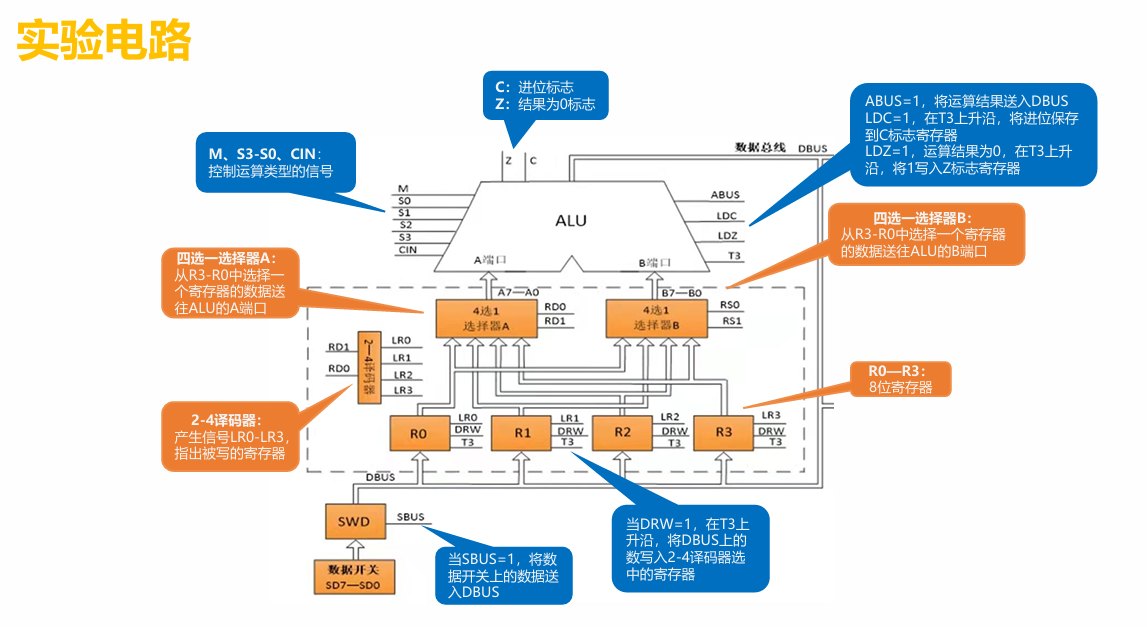
\includegraphics[width=15 cm]{1_cu.jpg}
        \end{figure}
        
        \par 一次完整的运算步骤的电路分析如下:
        \begin{enumerate}
            \item 通过数据开关 \textit{SD}7-\textit{SD}0 将两位 $16$ 进制数输入到 \textit{SWD} 中,当 $SBUS = 1$ 时,数据被送入 \textit{DBUS} 总线上
            \item 通过 2-4 译码器片选输入 $RD0$、$RD1$ 进行寄存器的选择
            \item 令 $DRW = 1$,此时被选中的寄存器可以写入
            \item 按下 $QD$ 输入时钟信号,在 $T3$ 时钟上升沿 \textit{DBUS} 中的数据被写入寄存器中
            \item 重复,将所需数据全部存入寄存器后,关闭 \textit{DRW}, 通过 4 选 1 数据选择器 A、B 输入 $RD0$、$RD1$、$RS0$、$RS1$ 将对应寄存器中的数据输入至 \textit{ALU} 的 \textit{A} 端口和 \textit{B} 端口
            \item 通过 $M$、$S3$-$S0$、$CIN$ 选择运算器的运算模式,关闭 \textit{SBUS},开启 \textit{ABUS},可以将计算结果送入 $DBUS$ 中。其中,当 $LDC = 1$ 时,将进位标志输入 $C$ 标志寄存器中;当 $LDZ = 1$ 时,将零标志输入 $Z$ 寄存器中
            \item 按下 $QD$,计算结果在 $T3$ 时钟上升沿被送入 \textit{DBUS} 中  
        \end{enumerate}

    \subsection{思考题解答}
        \begin{problem}
            是否能将 \textit{ALU} 的运算结果存入寄存器 $R3$ 中?WHYYYYYY?
        \end{problem}
        \begin{solution}
            当且仅当运算器 \textit{A} 端口的输入是 $R3$ 寄存器中的数据时可以。其他情况,由电路图可知,$RD0$、$RD1$ 同时负责选中输入 $A$ 端口的寄存器和2-4译码器的片选,由于 \textit{ALU} 是组合逻辑电路,一旦改变选中的寄存器为 $R3$ 输入和输出的值会立刻发生改变
        \end{solution}

    \subsection{实验过程及结果}
        \subsubsection{实验过程记录表}
            \begin{table}[htbp]
                \centering
                \scalebox{0.5}{
                \begin{tabular}{|c|>{\centering\arraybackslash}p{4cm}|c|c|>{\centering\arraybackslash}p{3cm}|c|}
                    \hline
                    \multicolumn{6}{|c|}{\textbf{运算器组成实验}} \\ \hline
                    \textbf{序号} & \textbf{操作} & \textbf{数据开关} & \textbf{操作目的} & \textbf{实验现象} & \textbf{备注} \\ \hline
                    \textbf{1} & CLR & & 复位 & & \\ \hline
                    \textbf{2} & DP=1 & & 设置操作模式 & & \\ \hline
                    \textbf{3} & SBUS=1 & 0FH & 将 0FH 送入 DBUS 上 & D7-D0=0FH & \multirow{12}{*}{向通用寄存器堆内的R3-R0置入数据} \\ \cline{1-5}
                    \textbf{4} & RD1=0, RD0=0 & & 选中 R0 寄存器 & D7-D0=0FH & \\ \cline{1-5}
                    \textbf{5} & DRW=1, QD & & 将 DBUS 上的数据写入寄存器 R0 中 & D7-D0=0FH A7-A0=0FH & \\ \cline{1-5}
                    \textbf{6} & SBUS=1 & 10H & 将 10H 送入 DBUS 上 & D7-D0=10H & \\ \cline{1-5}
                    \textbf{7} & RD1=0, RD0=1  & & 选中 R1 寄存器 & D7-D0=10H & \\ \cline{1-5}
                    \textbf{8} & DRW=1, QD & & 将 DBUS 上的数据写入寄存器 R1 中 & D7-D0=10H A7-A0=10H & \\ \cline{1-5}
                    \textbf{9} & SBUS=1 & 03H & 将 03H 送入 DBUS 上 & D7-D0=03H & \\ \cline{1-5}
                    \textbf{10} & RD1=1, RD0=0 & & 选中 R2 寄存器 & D7-D0=03H & \\ \cline{1-5}
                    \textbf{11} & DRW=1, QD & & 将 DBUS 上的数据写入寄存器 R2 中 & D7-D0=03H A7-A0=03H & \\ \cline{1-5}
                    \textbf{12} & SBUS=1 & 05H & 将 05H 送入 DBUS 上 & D7-D0=05H & \\ \cline{1-5}
                    \textbf{13} & RD1=1, RD0=1 & & 选中 R3 寄存器 & D7-D0=05H & \\ \cline{1-5}
                    \textbf{14} & DRW=1, QD & & 将 DBUS 上的数据写入寄存器 R3 中 & D7-D0=05H A7-A0=05H & \\ \hline
                    \textbf{15} & S3-S0=FH, M=1, CIN=0, RD1=0, RD0=0, ABUS=1 & & 将 R0 的数据送入 DBUS 上 & D7-D0=0FH A7-A0=0FH & 读取寄存器中的数据 \\ \hline
                    \textbf{16} & S3-S0=9H, M=0, CIN=1, RS1=1, RS0=0, ABUS=1 & & 选中 R1(B), R0(A)在上一步已选中,加法运算 10F+0FH & D7-D0=1FH, A7-A0=0FH, B7-B0=10H & \\ \hline
                    \textbf{17} & S3-S0=6H, M=1, CIN=0, ABUS=1 & & 减法运算, 0FH-10H & D7-D0=FFH & \\ \hline
                    \textbf{18} & S3-S0=BH, M=1, CIN=0, ABUS=1 & & 与运算, 0FH\&10H & D7-D0=00H & \\ \hline
                    \textbf{19} & S3-S0=EH, M=1, CIN=0, ABUS=1 & & 或运算, 0FH|10H & D7-D0=1FH & \\ \hline
                \end{tabular}
                } 
            \end{table}
            \begin{table}[htbp]
                \centering
                \begin{tabular}{|c|c|c|c|c|c|c|}
                    \hline
                    \multicolumn{7}{|c|}{\textbf{实验数据记录表}} \\ \hline
                    \multicolumn{2}{|c|}{\textbf{实验数据}} & \multicolumn{2}{c}{\textbf{实验过程}} & \multicolumn{3}{|c|}{\textbf{实验结果}} \\ \hline
                    \textbf{A} & \textbf{B} & \textbf{操作} & \textbf{控制信号} & \textbf{数据结果} & \textbf{C} & \textbf{Z} \\ \hline
                    0FH & 10H & A ++ & M=0, S3-S0=0H, CIN=0 & 10H & 0 & 0 \\ \hline
                    0FH & 10H & A + B & M=0, S3-S0=9H, CIN=1 & 1FH & 0 & 0 \\ \hline
                    0FH & 10H & A - B & M=0, S3-S0=6H, CIN=0 & FFH & 0 & 0 \\ \hline
                    0FH & 10H & A \& B & M=1, S3-S0=BH, CIN=0 & 00H & 0 & 0 \\ \hline
                    0FH & 10H & A | B & M=1, S3-S0=EH, CIN=0 & 1FH & 0 & 0 \\ \hline
                \end{tabular}  
            \end{table}
    \subsection{实验收获及体会}
        \par 理解了计算机进行计算的基本流程和ALU的运算原理



